\documentclass[a4paper]{article}
\usepackage[a4paper,%
    text={180mm, 260mm},%
    left=15mm, top=15mm]{geometry}
\usepackage[utf8]{inputenc}
\usepackage{cmap}
\usepackage[english, russian]{babel}
\usepackage{indentfirst}
\usepackage{amssymb}
\usepackage{amsmath}
\usepackage{mathtools}
\usepackage{tcolorbox}
\usepackage{graphicx}
\graphicspath{ { ./figures/ } }

\begin{document}
    \begin{center}
        \underline{УМФ. Лекция}
    \end{center}

\begin{equation}
    \sum\limits_{i,j  = 1}^{n}  a_{ij} \frac{\partial^2 u}{\partial x_i \partial x_j} 
    + \sum\limits_{i=1}^{n} a_i \frac{\partial u}{\partial x_i} + au(x) = f(x)
\end{equation}

Замена:
\begin{equation}
    \xi_k = \sum\limits_{i=1}^{n} c_{ki} x_i, \quad k=\overline{1,n}
\end{equation}

\[
    \tilde{u}(\xi_1, \dots \xi_n) = u(x_1, \dots x_n)
\]
\[
    \frac{\partial u}{\partial x_i} = \sum\limits_{k = 1}^{n} \frac{\partial u}{\partial \xi_k}  
    \frac{\partial \xi_k}{\partial x_i} = \sum\limits_{k=1}^{n} c_{ki} 
    \frac{\partial \tilde{u}}{\partial \xi_k} 
\]
\[
    \frac{\partial ^2 u}{\partial x_i \partial x_j} = \sum\limits_{k=1}^{n} 
    c_{ki} \frac{\partial }{\partial x_j} (\frac{\partial \tilde{u}}{\partial \xi_k} 
    = \sum\limits_{k=1}^{n}  c_{ki} \sum\limits_{l=1}^{n} \frac{\partial ^2 \tilde{u}}
    {\partial \xi_k \partial \xi_l} \frac{\partial \xi_l}{\partial x_j}  =
    \sum\limits_{k, l = 1}^{n}  c_{ki}c_{lj} \frac{\partial ^2 \tilde{u}}
    {\partial \xi_k \partial \xi_l}
\] 

\begin{equation}
    \tilde{a}_{kl} = \sum\limits_{i, j =1}^{} a_{ij}c_{ki}c_{lj}
\end{equation}


\begin{equation}
    \begin{aligned}
        \sum\limits_{i,j=1}^{n} a_{ij}t_i t_j = \sum\limits_{k,l}^{} \tilde{a}_{kl}
        \tau_k \tau_l \\
        t_i = \sum\limits_{k=1}^{n} c_{ki} \tau_k \\
        t_j = \sum\limits_{l=1}^{n} c_{lj} \tau_l
    \end{aligned}
\end{equation}

$ a_{kk} \in \{1;-1;0\} \quad \tilde{a}_{kl} = 0, \; k \neq l $ - Канонический вид \\
Если $ \tilde{a}_{kk} = 1 \; (a_{kk}  = -1), \; k=1,\dots, n $ - Уравнение
эллиптического вида \\
$ n-1 \text{ коэф } +1 \\
1  - -1$ \\
$ n-1 \text{ коэф } -1 \\
1  - +1$ \\
\textbf{\underline{Def}} \\
Если есть 1 и -1 и их не менее двух - уравнение ультрагиперболичекского типа\\
\textbf{\underline{Def}}  \\
Уравнение имеет параболический тип, если среди $ a_{kk} $ есть хотя бы один 0,
а все ненулевые коэф-ты одного знака \\

Если все собственные числа одного знака и нулей нет - уравнение эл.типа \\
Есть разного знака ??? - гипер тип \\
Если есть ноль остальные одного знака - параб тип

\section*{\centering Уравнения гиперболического типа}
Вопрос с билета: Вывод ур-я малых поперечных колебаний струны \\
u - отклонение точки струны x в момент времени t от поперечного сечения?  \\
$ |u_x| << 1 $ \\
Струна не оказывает сопротивление изгибу и ёё взаимодейтсвие с соседними участками
опр-ся только силами натяжения, касательными к профилю струны\\
\begin{figure}
    \begin{center}
        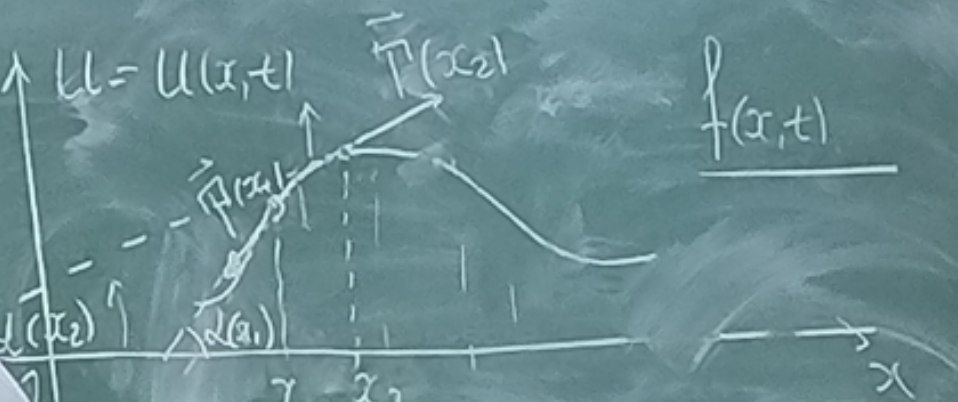
\includegraphics[width=0.95\textwidth]{./figures/fig1-2.png}
    \end{center}
    \caption{Поперечное изображение струны}
\end{figure}


$ l = \int\limits_{x_1}^{x_2} \sqrt{1+u^2} = x_1 - x_2 $ \\
Силы натяжения не зависят от времени(Закон Гука) \\
Задана $ f(x,t) $ - проекция на ось u линейной плотности сил \\
\[
    \int\limits_{x_1}^{x_2} f(x,t) dx = \vec{F}(t)
\]
Закон Ньютона в проекциях:
\[
    T(x_2)\cos\alpha(x_2) - T(x_1)\cos\alpha(x_1) = 0
\]

$ \cos\alpha \approx 1 $, T независит от x\\

$\rho(x)$ - линейная плотность струны
\[
    \int\limits_{x_1}^{x_2} \rho(x) dx = m_{[x_1;x_2]}
\]
\[
    \rho \frac{\partial ^2 u(x,t)}{\partial t^2} \Delta x =
    T(\frac{\partial u}{\partial x}\big|_{x+\Delta x} - \frac{\partial u}
    {\partial x}\big|_{x}) + f(x,t)dx \Delta x
\]

$ \sin\alpha = \frac{\tg\alpha}{\sqrt{1+\tg^2\alpha}} $ 

\begin{equation}
    \rho \frac{\partial ^2 u}{\partial t^2} - T\frac{\partial ^2 u}{\partial x^2} = f(x,t)
\end{equation}
\begin{equation}
    u_{tt}(x,t) - a^2 u_{xx}(x,t) = F(x,t)
\end{equation}
\[
    a^2 = \frac{T}{\rho} \quad F = \frac{f}{\rho} 
\]
Если $ F \equiv 0 $ - невынужденные колебания \\
Если $ F \neq 0 $ - вынужденные колебания \\

Тоже уравнение задает малые продольные колебания стержня \\

\end{document}
